\documentclass[final]{beamer}
\mode<presentation>
\usetheme{IWH}
% Use the beamerposter package
%\usepackage[orientation=portrait,size=a1,scale=1.15]{beamerposter}


\usepackage[orientation=portrait,scale=1.15]{beamerposter}
\setlength{\paperwidth}{36in}
\setlength{\paperheight}{48in}
\setlength{\textwidth}{0.98\paperwidth}
\setlength{\textheight}{0.98\paperheight}
\usepackage{graphicx} % for including images
\usepackage{amsmath} % for math symbols
\usepackage{amssymb} % for more math symbols
\usepackage{amsfonts}
\usepackage{lmodern} % scalable font package
\usepackage{booktabs}
\usepackage{colortbl}
\usepackage{multirow}
\usepackage{multicol}
\usepackage{subcaption}
\usepackage{setspace}

% Define poster colors and style
\usepackage{color}
\definecolor{darkblue}{rgb}{0.1,0.1,0.5}
\setbeamercolor{title}{fg=darkblue}

%\usepackage[pdftex,hiresbb]{graphicx}
%\usepackage[pageshow]{xtab}
\usepackage[bottom,hang,splitrule]{footmisc}
\usepackage[font={small},labelfont={bf},textfont={bf},format=hang,justification=RaggedRight]{caption}
\usepackage{tabularx}
\usepackage{natbib}
%\usepackage[spaces,hyphens]{url}
\usepackage{breakcites}
\usepackage{fancyhdr}
\usepackage{longtable}
\usepackage{dcolumn}
\usepackage{booktabs}
\usepackage{hyphenat}
%\usepackage[hidelinks]{hyperref}
\usepackage{doi}
\usepackage[UKenglish]{babel}
\usepackage[pdftex]{rotating} % [counterclockwise] %evtl. miteinbinden
\usepackage{color}
\usepackage[section]{placeins}
%\usepackage{subfig}
\usepackage{siunitx}
\sisetup{detect-all}


%%%%%%%%%%%%%%%5
\usepackage{environ}% Required for \NewEnviron, i.e. to read the whole body of the environment
\makeatletter

\newcounter{acolumn}%  Number of current column
\newlength{\acolumnmaxheight}%   Maximum column height


% `column` replacement to measure height
\newenvironment{@acolumn}[1]{%
	\stepcounter{acolumn}%
	\begin{lrbox}{\@tempboxa}%
		\begin{minipage}{#1}%
		}{%
		\end{minipage}
	\end{lrbox}
	\@tempdimc=\dimexpr\ht\@tempboxa+\dp\@tempboxa\relax
	% Save height of this column:
	\expandafter\xdef\csname acolumn@height@\roman{acolumn}\endcsname{\the\@tempdimc}%
	% Save maximum height
	\ifdim\@tempdimc>\acolumnmaxheight
	\global\acolumnmaxheight=\@tempdimc
	\fi
}

% `column` wrapper which sets the height beforehand
\newenvironment{@@acolumn}[1]{%
	\stepcounter{acolumn}%
	% The \autoheight macro contains a \vspace macro with the maximum height minus the natural column height
	\edef\autoheight{\noexpand\vspace*{\dimexpr\acolumnmaxheight-\csname acolumn@height@\roman{acolumn}\endcsname\relax}}%
	% Call original `column`:
	\orig@column{#1}%
}{%
	\endorig@column
}

% Save orignal `column` environment away
\let\orig@column\column
\let\endorig@column\endcolumn

% `columns` variant with automatic height adjustment
\NewEnviron{acolumns}[1][]{%
	% Init vars:
	\setcounter{acolumn}{0}%
	\setlength{\acolumnmaxheight}{0pt}%
	\def\autoheight{\vspace*{0pt}}%
	% Set `column` environment to special measuring environment
	\let\column\@acolumn
	\let\endcolumn\end@acolumn
	\BODY% measure heights
	% Reset counter for second processing round
	\setcounter{acolumn}{0}%
	% Set `column` environment to wrapper
	\let\column\@@acolumn
	\let\endcolumn\end@@acolumn
	% Finally process columns now for real
	\begin{columns}[#1]%
		\BODY
	\end{columns}%
}
\makeatother
%%%%%%%%%%

% Title, author, and date
\title{Smooth and Persistent Forecasts of German GDP}
%\subtitle[]{\hspace{1.9cm}\LARGE{ A quarterly evaluation of EU Commissions' GDP forecasts}}

\author[]{Katja Heinisch$^{\textit{ 1}}$, Simon van Norden$^{\textit{ 2}}$, Marc Wildi$^{\textit{ 3}}$}
\institute[IWH]{\normalsize{$^{\textit{1}}$ Halle Institute for Economic Research (IWH), $^{\textit{2}}$ HEC Montréal and CIREQ, $^{\textit{3}}$ Zurich University of Applied Sciences (ZHAW) }}
%\author[]{Katja Heinisch}
%\institute[IWH]{Halle Institute for Economic Research}
%\vspace{2cm}


\begin{document}
	
	\begin{frame}
		\begin{columns}[T]
			% Column 1
			\begin{column}{0.48\textwidth}
					\begin{block}{\large Motivation}
								
					\begin{itemize}
					\item Forecasting dilemma: Efficiency requires full use of information, yet resulting forecasts are often highly volatile.
				%	Trade-off between informational efficiency and forecast smoothness.
					\item Short-term volatility and data revisions challenge reliable forecasting.
				\item \cite{Wildi2024,Wildi2025,McElroy2019,McElroy2020} propose the Smooth Sign Accuracy (SSA) framework, which controls volatility via penalizing forecast sign changes.
				\\
				\vspace{1cm}
					 {\textbf{\textcolor{iwhdarkblue}{Research Questions:}}}
			
					\item Can we improve GDP forecast smoothness without sacrificing accuracy?
					\item Do filtering techniques enhance persistence and coherence?
                    \begin{itemize}
                    \begin{normalsize}
                        \item Replace raw leading indicators with smoothed and filtered components 
                         \item Improve the signal-to-noise ratio. 
                    \end{normalsize}
                 \end{itemize}
                    \end{itemize}
			
			\end{block}
					
		\begin{block}{\large Data}
															
					  \begin{columns}[T]
						\column{0.495\textwidth}
							\begin{itemize}
							     \item Quarterly German GDP (1995–2024).
							     \item Monthly Indicators: Industrial Production, ifo Business Climate, ESI, Term spread 10y-3m.
							     \item Log-differenced, standardized (except spreads), outliers trimmed (COVID-19).
							     \item Data aligned to account for publication lags and converted to quarterly frequency 
							     \item Dynamic dependencies are explored via cross-correlation functions (CCFs) and vector moving-average (VMA) representations.
							     \item Survey indicators show strong leading correlations with GDP; IP and term spread exhibit weaker or delayed effects.
							     \item Pandemic-related outliers distort dynamic patterns; hence, data from Q4-2019 to Q4-2020 are excluded for stability.
							\end{itemize}
								   							  	
						\column[T]{0.495\textwidth}
									\begin{center}{\small{\textbf{\textcolor{black}{Figure 1: Leads \& lags}}}}
									
									    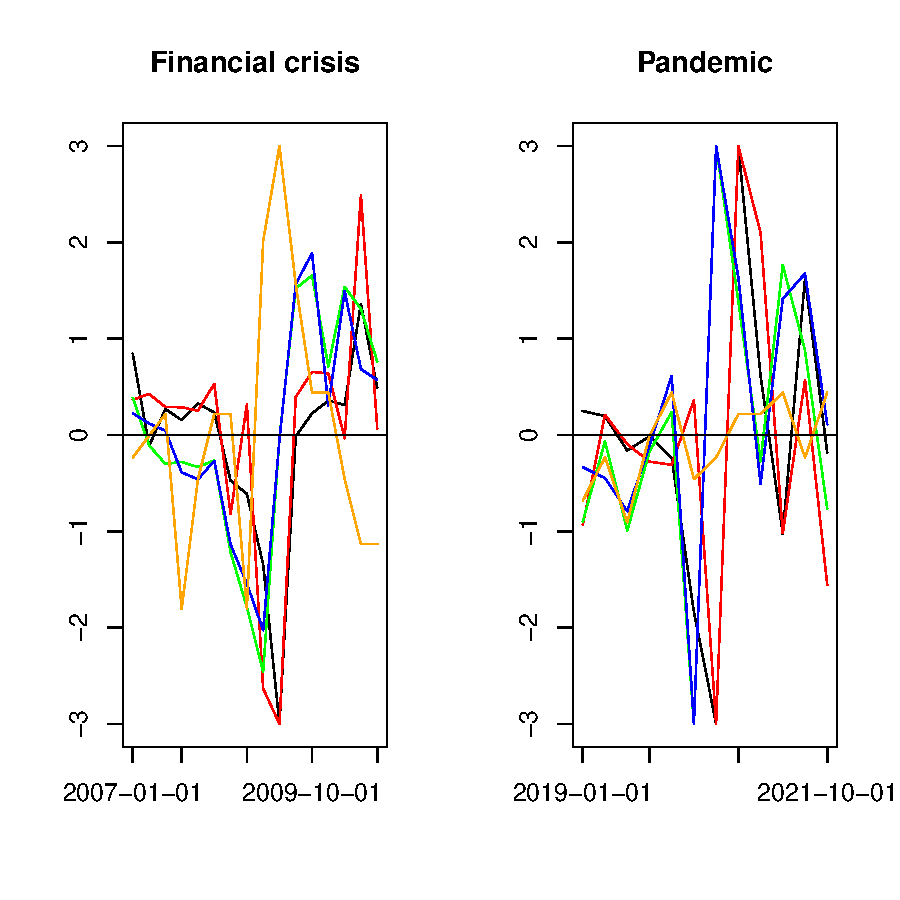
\includegraphics[width=1\textwidth]{./Figures/data_lags.pdf}
									\end{center}
\vspace{-1cm}
								\leftskip2em \singlespacing{ {\footnotesize \emph{Note:} GDP \& Indicators:  GDP (blue), IP (red), ifo (green), ESI (blue) and term-spread (yellow). Data standardized log-differences, trimmed to $\pm 3$ standard deviations.} }
						\end{columns}
				
			
					
				\end{block}
				
		\begin{block}{\large{Direct Forecasts}}
			\begin{itemize}
				\item Regression of GDP on contemporaneous indicators.
				\item Lead/lag structure motivates the use of multivariate models to improve forecast accuracy.
				\item As the forecast horizon $h$ increases, the turning points (i.e., peaks and troughs) of the direct forecasts become increasingly right-shifted (lagging). 
			\end{itemize}
		
		\begin{columns}[T]
			\column{0.495\textwidth}
				\\
				\vspace{1cm}					
				\textcolor{iwhdarkblue}{\textbf{Filtering Indicators: HP}}
					\begin{itemize}
						\item Forecasts are re-estimated using indicators smoothed via the one-sided HP-C filter (HP(160)).
						\item Figures show improved alignment: forecasts lag GDP less and better capture turning points.
						\item Filtering reduces high-frequency noise and enhances signal extraction.
					\end{itemize}
				\begin{footnotesize}
						\begin{table}[h]
						\begin{center}
								{\small{\textbf{\textcolor{black}{Table 1: }}}}
                                \\
				\vspace{0.3cm}
                            \begin{tabular}{lrrrrrrr}
							\hline
							& h= 0 & h= 1 & h= 2 & h= 3 & h= 4 & h= 5 & h= 6 \\ 
							\hline
							Unfiltered & 0.028 & 0.000 & 0.001 & 0.910 & 0.509 & 0.091 & 0.178 \\ 
							HP-C filtered & 0.000 & 0.001 & 0.036 & 0.046 & 0.049 & 0.012 & 0.022 \\ 
							\hline
						\end{tabular}
						\leftskip2em \singlespacing{ {\footnotesize \emph{Note:} p-values for $H_0: \hat{\beta} = 0$, HAC-adjusted Wald test.\\Estimation over full sample (without pandemic).					\label{tab:pvaluedhp}}}
						\end{center}
						\end{table}
				\end{footnotesize}
			\begin{itemize}
				\item HP-C filter improves smoothness but remains univariate and prone to high-frequency leakage.
			\end{itemize}
		
			
				\column{0.495\textwidth}
									
				\begin{center}
				{\small{\textbf{\textcolor{black}{Figure 2: Performance of direct forecasts}}}}
				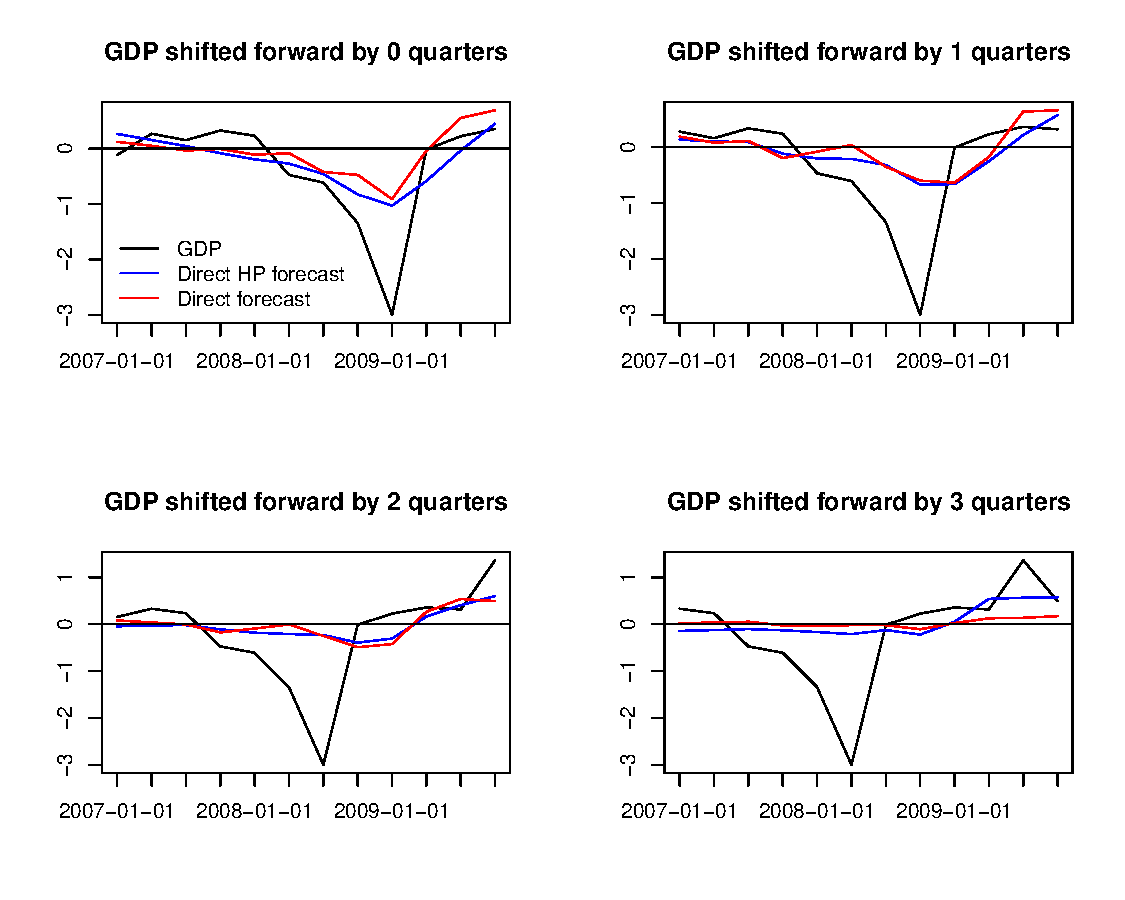
\includegraphics[width=1\textwidth]{./Figures/direct_hp_forecasts_financial_crisis.pdf}
				\end{center}
			
				\end{columns}	
			\end{block}		
			
				\begin{block}{\large Empirical Approach -- Multivariate Smooth Sign Accuracy (M-SSA)}
						\addtolength{\itemsep}{10pt}
			%	\textcolor{iwhdarkblue}{\textbf{Filtering Indicators}}
            \begin{columns}[T]
			\column{0.495\textwidth}
            
				\begin{itemize}
				 
				\item M-SSA extends SSA \citep{Wildi2025} to multivariate setting with causal (one-sided) filters.
				\item Target variable $z_t$ (e.g. HP-GDP) is tracked by predictor $y_t$ via multivariate filters on leading indicators.
				\item SSA criterion: maximize forecast-target correlation under constraint on forecast autocorrelation $\rho(y,1)$.
				\item Constraint controls smoothness via expected holding time: $ht(y) = \frac{\pi}{\arccos(\rho(y,1))}$.
				\item Optimization via constraints on sign-changes.
			\end{itemize}
            \column{0.495\textwidth}
									
				\begin{center}
				{\small{\textbf{\textcolor{black}{Figure 3: M-SSA vs. HP-C}}}}
				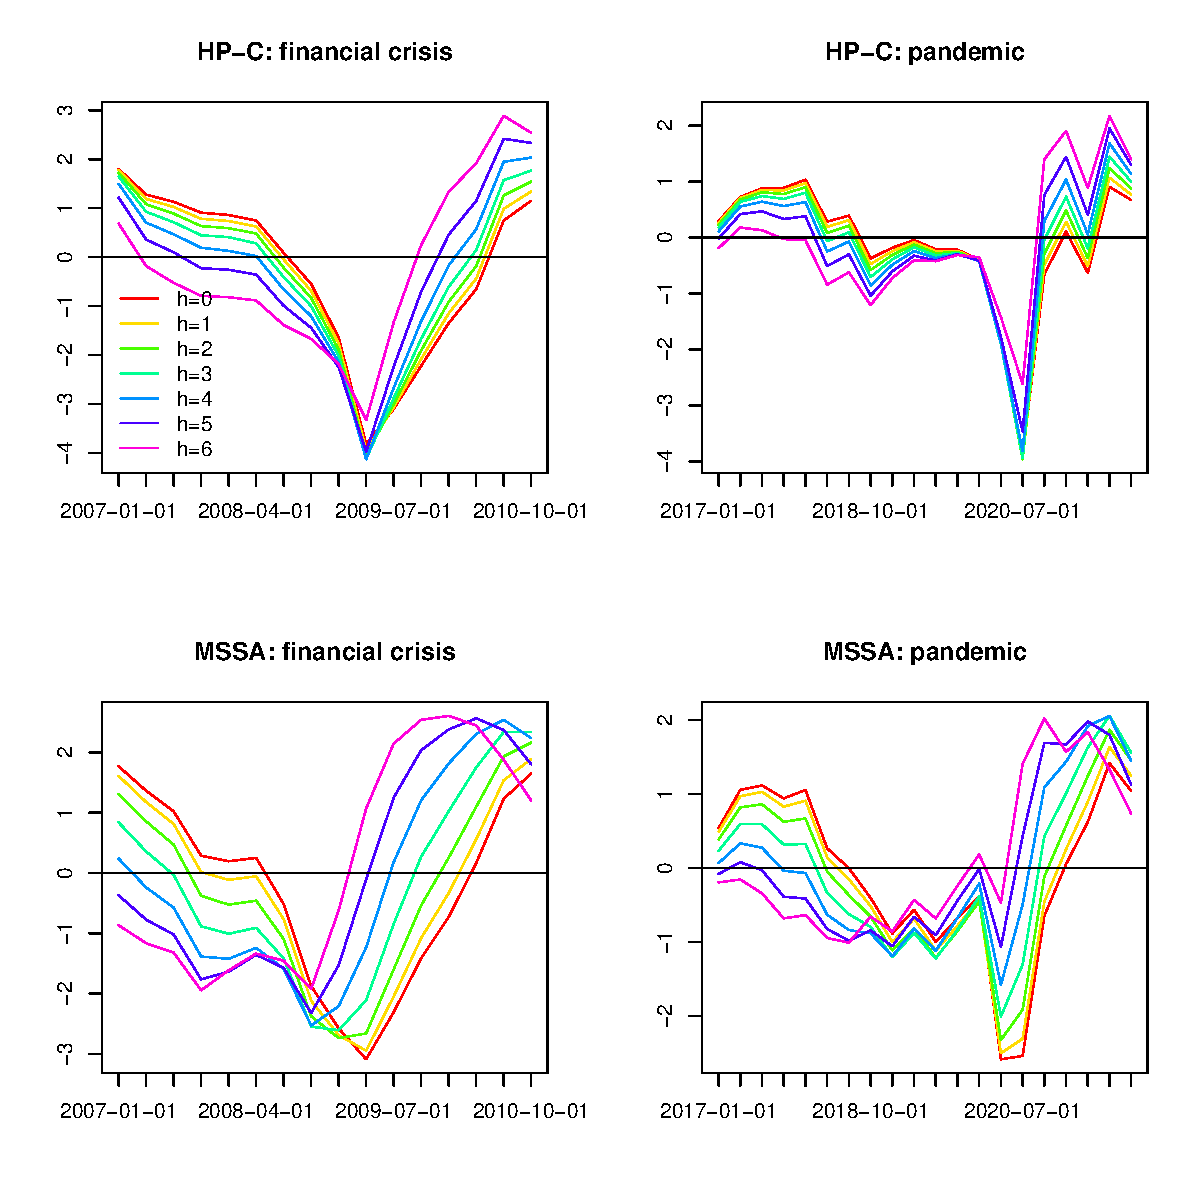
\includegraphics[width=1\textwidth]{./Figures/multivar_vs_univar.pdf}
				\end{center}
			
				\end{columns}	
            \begin{itemize}
				 
				\item In contrast to HP (top two panels Figure 3), the multivariate filter (lower two panels) can track recession dips as the forecast horizon increases.
                \item Main explanation for improved forecast performances at larger horizons ($h>2$).
			\end{itemize}
%	\autoheight
			\end{block}
				
			\end{column}
		%%%%%%%%%%%%%%%%%%%%%%%%%%%%%%%%%%%%%%%%%%%%%%%%%%%%%%
			% Column 2
		\begin{column}{0.48\textwidth}
			
			\begin{block}{\large{Results}}
				
			\begin{columns}[T]
			\column{0.495\textwidth}
			\textcolor{iwhdarkblue}{\textbf{M-SSA Nowcasts vs M-MSE}}\\
			\begin{itemize}
			\item Comparison of nowcasts for HP-GDP using M-SSA vs M-MSE.
			\item M-SSA reduces sign changes by 33\% with minimal loss of accuracy.
			\item M-SSA achieves longer holding times: a $50\%$ increase compared to M-MSE.
			\end{itemize}
		
		\column{0.495\textwidth}
			  \begin{center}
			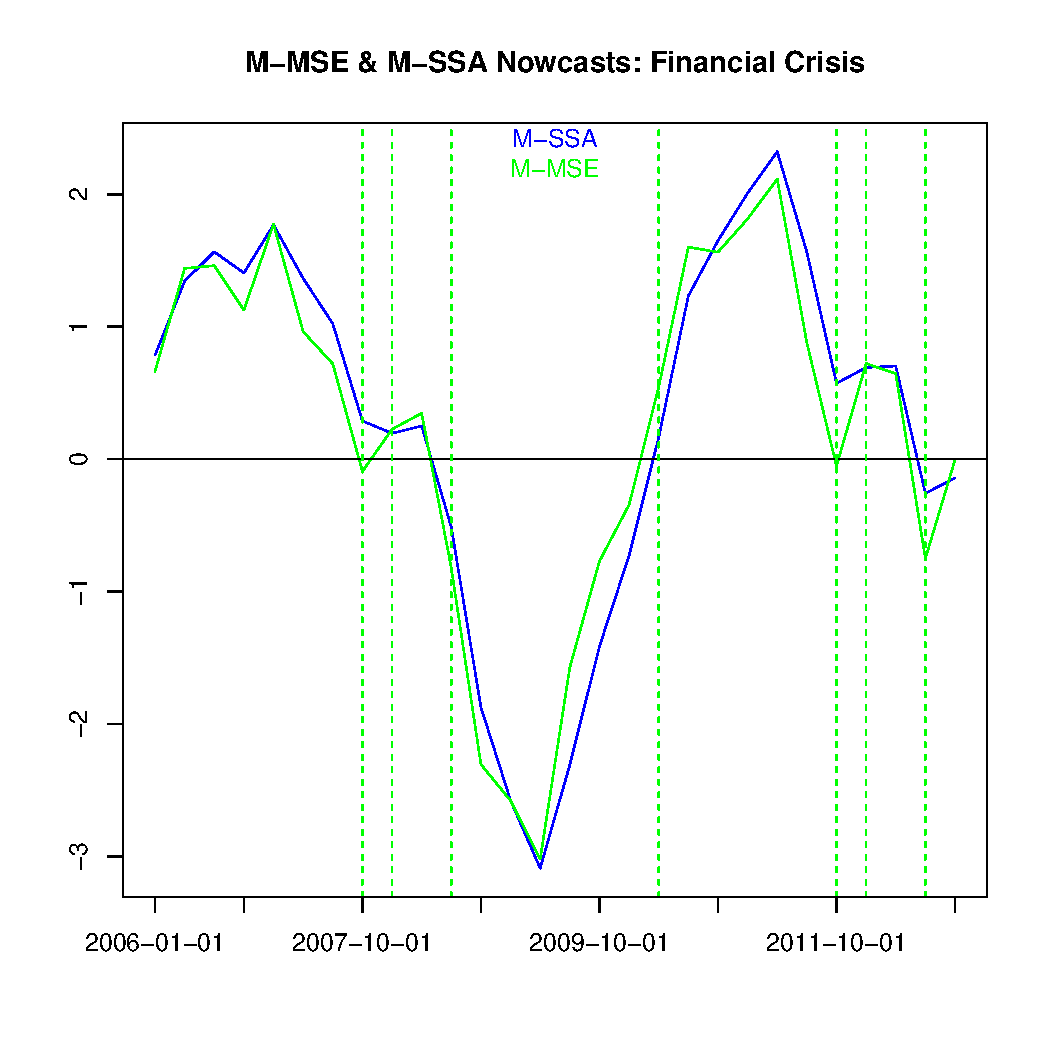
\includegraphics[width=0.8\textwidth]{./Figures/mssa_msse_zc.pdf}
				\leftskip2em \singlespacing{ {\footnotesize \emph{Note:} Nowcasts: M-SSA (blue) and M-MSE (green). \\The vertical green lines indicate sign changes of M-MSE  \\M-SSA (blue) has less zero-crossings (smoother).
				\label{mssa_msse_now}}}
		\end{center}
		\end{columns}
		
		
%					\vspace{1.5cm}
%					\textcolor{iwhdarkblue}{\textbf{M-SSA Forecasts for $h > 0$}}\\
%					
%						\begin{itemize}	
%								\addtolength{\itemsep}{10pt}	
%					\item M-SSA forecasts shift leftward consistently as $h$ increases, especially around turning points.
	
%						\end{itemize}	
				
			\vspace{1.5cm}
			
			\textcolor{iwhdarkblue}{\textbf{M-SSA Forecast}}\\
				\begin{itemize}
				\item Out-of-sample forecast performance is evaluated by comparing the M-SSA-based predictor to both a mean forecast and a direct forecast, all updated quarterly.
				
			\end{itemize}
			\begin{columns}
					\column{0.495\textwidth}
				
			\begin{itemize}
%			\item Out-of-sample forecast performance is evaluated by comparing the M-SSA-based predictor to both a mean forecast and a direct forecast, all updated quarterly.
			\item Results show that M-SSA predictors outperform both benchmarks at horizons larger than two quarters.
			\item Statistical significance of the M-SSA GDP predictor is confirmed for up to one year ahead, excluding the pandemic period.
			\end{itemize}
		
		
			\column{0.495\textwidth}
\begin{table}[ht]
	\centering
			{\small{\textbf{\textcolor{black}{Table 2: rRMSEs }}}}\\
              				\vspace{0.3cm}
\begin{footnotesize}
	\begin{tabular}{rrrrrrrr}
		\hline
		& h=0 & h=1 & h=2 & h=3 & h=4 & h=5 & h=6 \\ 
		\hline
Shift=0 & 0.973 & 0.937 & 0.888 & 0.850 & 0.855 & 0.900 & 0.956 \\ 
  Shift=1 & 1.073 & 1.051 & 0.997 & 0.918 & 0.870 & 0.873 & 0.906 \\ 
  Shift=2 & 1.069 & 1.077 & 1.063 & 1.006 & 0.940 & 0.907 & 0.907 \\ 
  Shift=3 & 1.020 & 1.045 & 1.066 & 1.048 & 0.997 & 0.957 & 0.941 \\ 
  Shift=4 & 0.983 & 1.016 & 1.056 & 1.064 & 1.023 & 0.974 & 0.942 \\ 
  Shift=5 & 0.988 & 1.026 & 1.071 & 1.088 & 1.057 & 1.007 & 0.963 \\
		\hline
	\end{tabular}
\end{footnotesize}
\begin{singlespace}
	\leftskip2em {\footnotesize \emph{Notes:}  Out-of-sample rRMSE of M-SSA vs. expanding mean forecast of GDP. Out-of-sample evaluation starting in Q1 2008, without pandemic.\\Values $< 1$ indicate superior predictions by M-SSA.}
\end{singlespace}
\vspace{0.5cm}
\end{table}





\begin{table}[ht]
	\centering
			{\small{\textbf{\textcolor{black}{Table 3: statistical significance}}}}\\
            \vspace{0.3cm}
\begin{footnotesize}
\begin{tabular}{rrrrrrrr}
  \hline
 & h=0 & h=1 & h=2 & h=3 & h=4 & h=5 & h=6 \\ 
  \hline
Shift=0 & 0.084 & 0.047 & 0.017 & 0.005 & 0.002 & 0.001 & 0.038 \\ 
  Shift=1 & 0.230 & 0.160 & 0.094 & 0.032 & 0.005 & 0.001 & 0.004 \\ 
  Shift=2 & 0.801 & 0.666 & 0.414 & 0.173 & 0.026 & 0.005 & 0.006 \\ 
  Shift=3 & 0.876 & 0.961 & 0.917 & 0.683 & 0.248 & 0.068 & 0.039 \\ 
  Shift=4 & 0.370 & 0.819 & 0.990 & 0.953 & 0.533 & 0.117 & 0.030 \\ 
  Shift=5 & 0.353 & 0.802 & 0.983 & 0.943 & 0.571 & 0.239 & 0.043 \\ 
   \hline
\end{tabular}
\end{footnotesize}
\begin{singlespace}
	\leftskip2em {\footnotesize \emph{Notes:} p-values for $H_0: \hat{\beta_1} = 0$, HAC-adjusted Wald test,\\sample excludes pandemic.}
\end{singlespace}
\vspace{0.5cm}
\end{table}

\end{columns}

\vspace{1.5cm}
\textcolor{iwhdarkblue}{\textbf{Receiver Operating Characteristic (ROC)}}\\
 \begin{columns}
    \column{0.495\textwidth}
      \begin{itemize}
			\item Compute hit rate and false alarm rate: ROC curve
            \item Performance measure: Area Under Curve (AUC)
			\end{itemize}



\begin{table}[ht]
	\centering
			{\small{\textbf{\textcolor{black}{Table 4: AUCs }}}}\\
            \vspace{0.3cm}
\begin{footnotesize}
\begin{tabular}{rrrrr}
  \hline
 & Direct & HP-C & M-MSE & M-SSA \\ 
  \hline
Forecast horizon 1 & 0.752 & 0.715 & 0.746 & 0.747 \\ 
  Forecast horizon 2 & 0.697 & 0.663 & 0.729 & 0.720 \\ 
  Forecast horizon 3 & 0.554 & 0.622 & 0.684 & 0.709 \\ 
  Forecast horizon 4 & 0.486 & 0.624 & 0.680 & 0.708 \\ 
  Forecast horizon 5 & 0.593 & 0.636 & 0.643 & 0.701 \\ 
   \hline
\end{tabular}
\end{footnotesize}
\begin{singlespace}
	{\footnotesize \emph{Notes:} AUCs of predictors against GDP at various forecast horizons.}
\end{singlespace}
\vspace{0.5cm}
\end{table}
            \begin{itemize}
			\item All filters outperform direct forecast (larger AUC) for $h>2$. 
            \item For $h>2$, M-SSA maximizes AUC, followed by M-MSE, HP-C and the direct forecast.
			\end{itemize}

    \column{0.495\textwidth}
        \begin{center}
        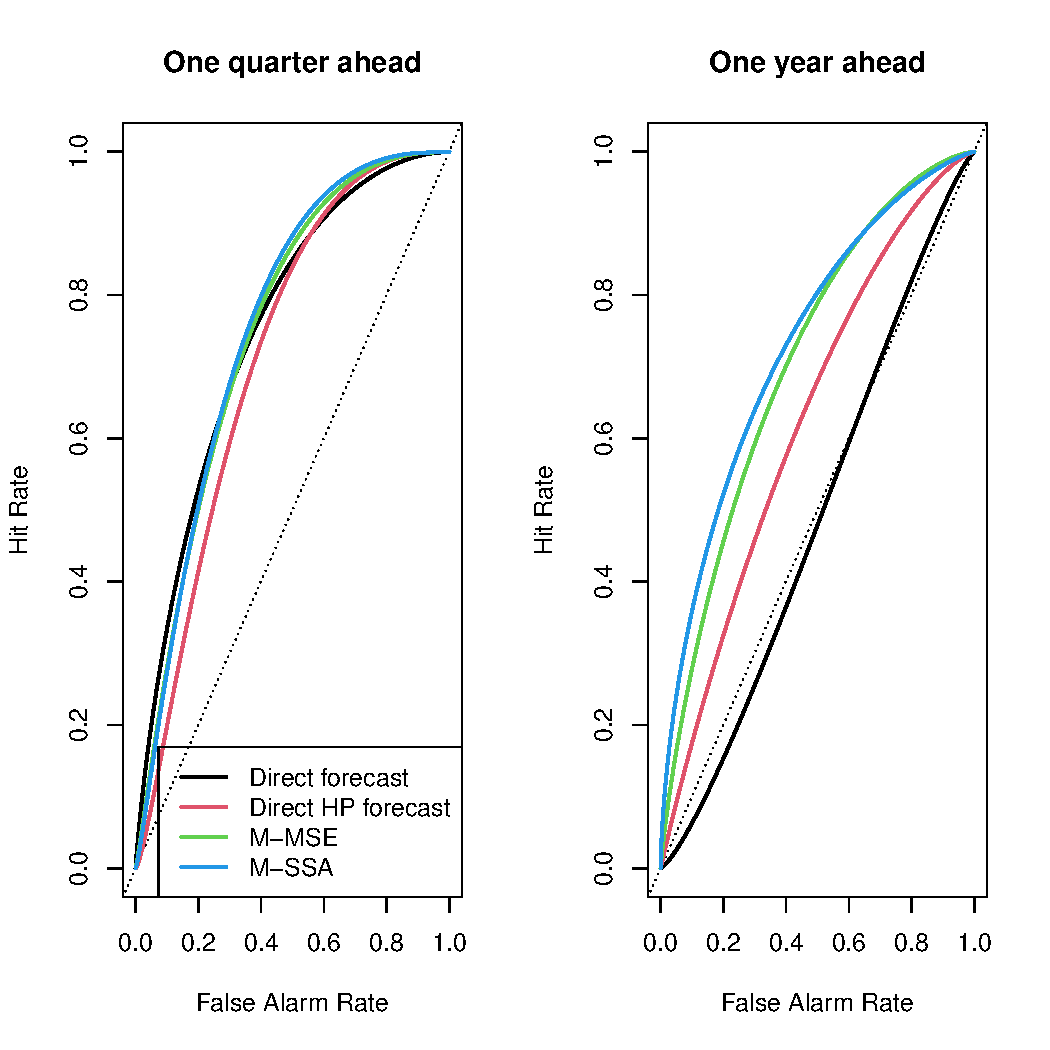
\includegraphics[width=0.8\textwidth]{./Figures/ROC_GDP_shift_1_4.pdf}
		
	     \end{center}
    
\end{columns}
   
			
			\end{block}
			
			\begin{block}{\large Summary and Conclusion}
				
			\begin{itemize}
            \item Classic direct forecasts of GDP outperform the mean benchmark up to two quarters ahead.  
            \item Smoothing with an HP(160)-filter improves performances at larger forecast horizons. But the filter cannot leverage leading indicators and remains noisy.
            \item To overcome these limitations, a multivariate SSA (M-SSA) framework based on \cite{Wildi2024} is introduced, leveraging cross-sectional indicator data and controlling the predictor’s zero-crossing rate for enhanced signal tracking at turning points.
            \item A simple regression of the M-SSA GDP component on future GDP yields a statistically significant predictor up to one year ahead, outperforming both mean benchmarks and classic direct forecasts at longer horizons.
            \item Stability in regression coefficients and filter design after a burn-in period improves the interpretability of the predictor, offering a robust integration of direct forecasting with multivariate signal extraction targeting quarterly GDP growth.
        \end{itemize}
			\end{block}
			
	
	
	 \begin{block}{\large References}
	\bibliographystyle{apalike}
    \begin{small}
        \bibliography{references}
          
        M-SSA package: https://github.com/wiaidp/R-package-SSA-Predictor    
        \end{small}
	
   
				%\end{flushright}
    \end{block}
		\end{column}
  
  
\end{columns}

\end{frame}

\end{document}
